%%%%%%%%%%%%%%%%%%%%%%%%%%%%%%%%%%%%%%%%%%%%%%%%%%%%%%%
%% Bachelor's & Master's Thesis Template             %%
%% Copyleft by Artur M. Brodzki & Piotr Woźniak      %%
%% Faculty of Electronics and Information Technology %%
%% Warsaw University of Technology, 2019-2020        %%
%%%%%%%%%%%%%%%%%%%%%%%%%%%%%%%%%%%%%%%%%%%%%%%%%%%%%%%

\documentclass[
    left=2.5cm,         % Sadly, generic margin parameter
    right=2.5cm,        % doesnt't work, as it is
    top=2.5cm,          % superseded by more specific
    bottom=3cm,         % left...bottom parameters.
    bindingoffset=6mm,  % Optional binding offset.
    nohyphenation=false % You may turn off hyphenation, if don't like.
]{meil/meil-thesis}


%\documentclass[
%    left=2.5cm,         % Sadly, generic margin parameter
%    right=2.5cm,        % doesnt't work, as it is
%    top=2.5cm,          % superseded by more specific
%    bottom=3cm,         % left...bottom parameters.
%    bindingoffset=6mm,  % Optional binding offset.
%    nohyphenation=false % You may turn off hyphenation, if don't like.
%]{eiti/eiti-thesis}

\langpol % Dla języka angielskiego mamy \langeng
\graphicspath{{img/}}             % Katalog z obrazkami.
\addbibresource{bibliografia.bib} % Plik .bib z bibliografią

\begin{document}

%--------------------------------------
% Strona tytułowa
%--------------------------------------
\MasterThesis % Dla pracy inżynierskiej mamy \EngineerThesis
%\PKR % Dla pracy inżynierskiej mamy \EngineerThesis
\instytut{Aerodynamiki}
\kierunek{Mechanika i Projektowanie Maszyn}
\specjalnosc{Modelowanie i Symulacje Komputerowe w Mechanice}
\title{
    Niepotrzebnie długi i skomplikowany tytuł pracy \\
    trudny do przeczytania, zrozumienia i wymówienia
}
\engtitle{ % Tytuł po angielsku do angielskiego streszczenia
    Unnecessarily long and complicated thesis' title \\
    difficult to read, understand and pronounce
}
\author{Paweł Gilewicz \\ Krystian Fudali}
\album{299058, 299057}
\promotor{dr inż. Tomasz Bobiński}
\date{\the\year}
\maketitle

%--------------------------------------
% Streszczenie po polsku
%--------------------------------------
%\cleardoublepage % Zaczynamy od nieparzystej strony
%\streszczenie \lipsum[1-3]
%\slowakluczowe XXX, XXX, XXX

%--------------------------------------
% Streszczenie po angielsku
%--------------------------------------
%\newpage
%\abstract \kant[1-3]
%\keywords XXX, XXX, XXX

%--------------------------------------
% Oświadczenie o autorstwie
%--------------------------------------
%\cleardoublepage  % Zaczynamy od nieparzystej strony
%\pagestyle{plain}
%\makeauthorship

%--------------------------------------
% Spis treści
%--------------------------------------
\cleardoublepage % Zaczynamy od nieparzystej strony
\tableofcontents

%--------------------------------------
% Rozdziały
%--------------------------------------
\cleardoublepage % Zaczynamy od nieparzystej strony
\pagestyle{headings}

\newpage % Rozdziały zaczynamy od nowej strony.
\section{Wstęp}

Odpowiedź kropli na wymuszenia o wysokich częstotliwościach jest problemem szeroko poruszanym w literaturze dotyczącej mechaniki płynów. Już Rayleigh w swoich pracach zajmował się wyznaczeniem modów drań kropli nielepkiej. Następni badacze Lamb / ktoś jeszcze rozwinęli teorię drgań kropli o przypadek uwzględniający lepkość. Obecnie analiza odpowiedzi kropli jest przedmiotem wielu prac eksperymentalnych. Badania dotyczą zarówno kropli rozlanej na powierzchni jak i kropli niepodpartej jako, że przypadki te znacznie się od siebie różnią. Przykładem analizy kropli podpartej jest eksperyment (autor) gdzie kroplę umieszczono na płytce wprawionej w pionowe drgania wysokiej częstotliwości przy pomocy głośnika. Prowadzenie takich rozważań pozwala na wyznaczenie częstości własnych i postaci drań kropli płynu. 



\subsection{Cel pracy magisterskiej}

Poniższa praca ma na celu zbadanie przypadku znacznie rzadziej spotykanego w literaturze. Zajęto się kroplą rozlaną na płytce wibrującej w płaszczyźnie poziomej. Celem pracy jest budowa stanowiska pozwalającego na zbadanie odpowiedzi kropli na wymuszenia ruchem płytki o wysokiej częstotliwości. Przez odpowiedź kropli na wymuszanie rozumiano zmianę jej kształtu, kąty zwilżania, a także moment wystąpienia uślizgu kropli.


\subsection{Opis zagadnienia}

Na rysunkyu 1.1 pokazano ilustracje badanego zagadnienia. Obszar $\Omega_w$ to kropla wody, obszar $\Omega_p$ powietrze. Płytka oznaczona symbolem $\Gamma$ porusza się z prędkością $\overrightarrow{v}$ zmienną w czasie. 
\begin{figure}[!h]
    \label{fig:poślizg}
    \centering 
\includegraphics[width=\linewidth]{img/mv.png}
    \caption{Zagadnienia}
\end{figure}

\subsubsection{Kąty zwilżania}
Głównym obiektem zainteresowania były kąty zwilżania kropli rozlanej na płytce. Kąt zwilżania definiowano jako kąt tworzony przez styczną do konturu kropli w punkcie kontaktu z płytką i płaszczyznę poziomą. Tak zdefiniowany kąt łatwo wyznaczyć na dwuwymiarowym obrazie kropli, jak pokazano na rysunku 1.2.

\begin{figure}[!h]
    \label{fig:kąt_zwilżania}
    \centering 
\includegraphics[width=0.9\linewidth]{img/kat_zwilzania.png}
    \caption{Kąty zwilżania}
\end{figure}

Podczas horyzontalnego ruchu płytki, zarówno kąt z lewej strony $\varphi_l$ jak i ten z prawej $\varphi_r$ zmieniają swoje wartości. Zagadnienie polega na wyznaczeniu tej zmienności w czasie i skorelowanie jej z częstotliwością i amplitudą drgań wymuszenia.\\


\subsubsection{Poślizg kropli}
Dla każdej amplitudy drgań płytki istnieje graniczna częstotliwość przy, której, poza zmianą kąta zwilżania, zmienia się także położenie kropli względem płytki. Inaczej kropla zaczyna się uślizgiwać i przesuwać po płytce. W pracy starano się wyznaczyć dla jakich częstotliwości i amplitud wystąpi uślizg. Sam moment, w którym kropla zaczyna się przesuwać nie jest łatwy do wyznaczenia. W poniższej pracy zakładano, że poślizg występuje gdy długość kontaktu kropli z płytką oznaczona $l$ zaczyna się zmieniać względem położenia statycznego. Moment poślizgu i długość $l$ pokazano na ilustracji 1.3.


\begin{figure}[!h]
    \label{fig:poślizg}
    \centering 
\includegraphics[width=0.9\linewidth]{img/poslizg.png}
    \caption{Uślizg kropli}
\end{figure}

\newpage

\section{Opis Stanowiska}
    Aby badać zmienność kątów zwilżania i poślizg zaprojektowano i przygotowano stanowisko pomiarowe. W celu rejestrowania kształtu kropli posłużono się kamerą o dużej częstotliwości rejestrowania klatek. Otrzymywany obraz z kamery jest 2 wymiarowy co pozwala w łatwy sposób zdefiniować kąty zwilżania. Do wprawiania płytki z kroplą w ruch wykorzystano wózek połączony z silnikiem liniowym \textit{Linmot} C1100. Wózek osadzono na łożyskach liniowych aby zapewnić płynność ruchu. Za wózkiem umieszczono silną lampę LED, która zapewnia dobre doświetlenie obrazu otrzymywanego z kamery. Na stanowisko składają się zatem następujące elementy:
    \begin{enumerate}
        \item kamera,
        \item sterownik silnika,
        \item silnik liniowy,
        \item lampa LED,
        \item łożyskowany wózek z płytką.
    \end{enumerate}

\begin{figure}[!h]
    \label{fig:poślizg}
    \centering 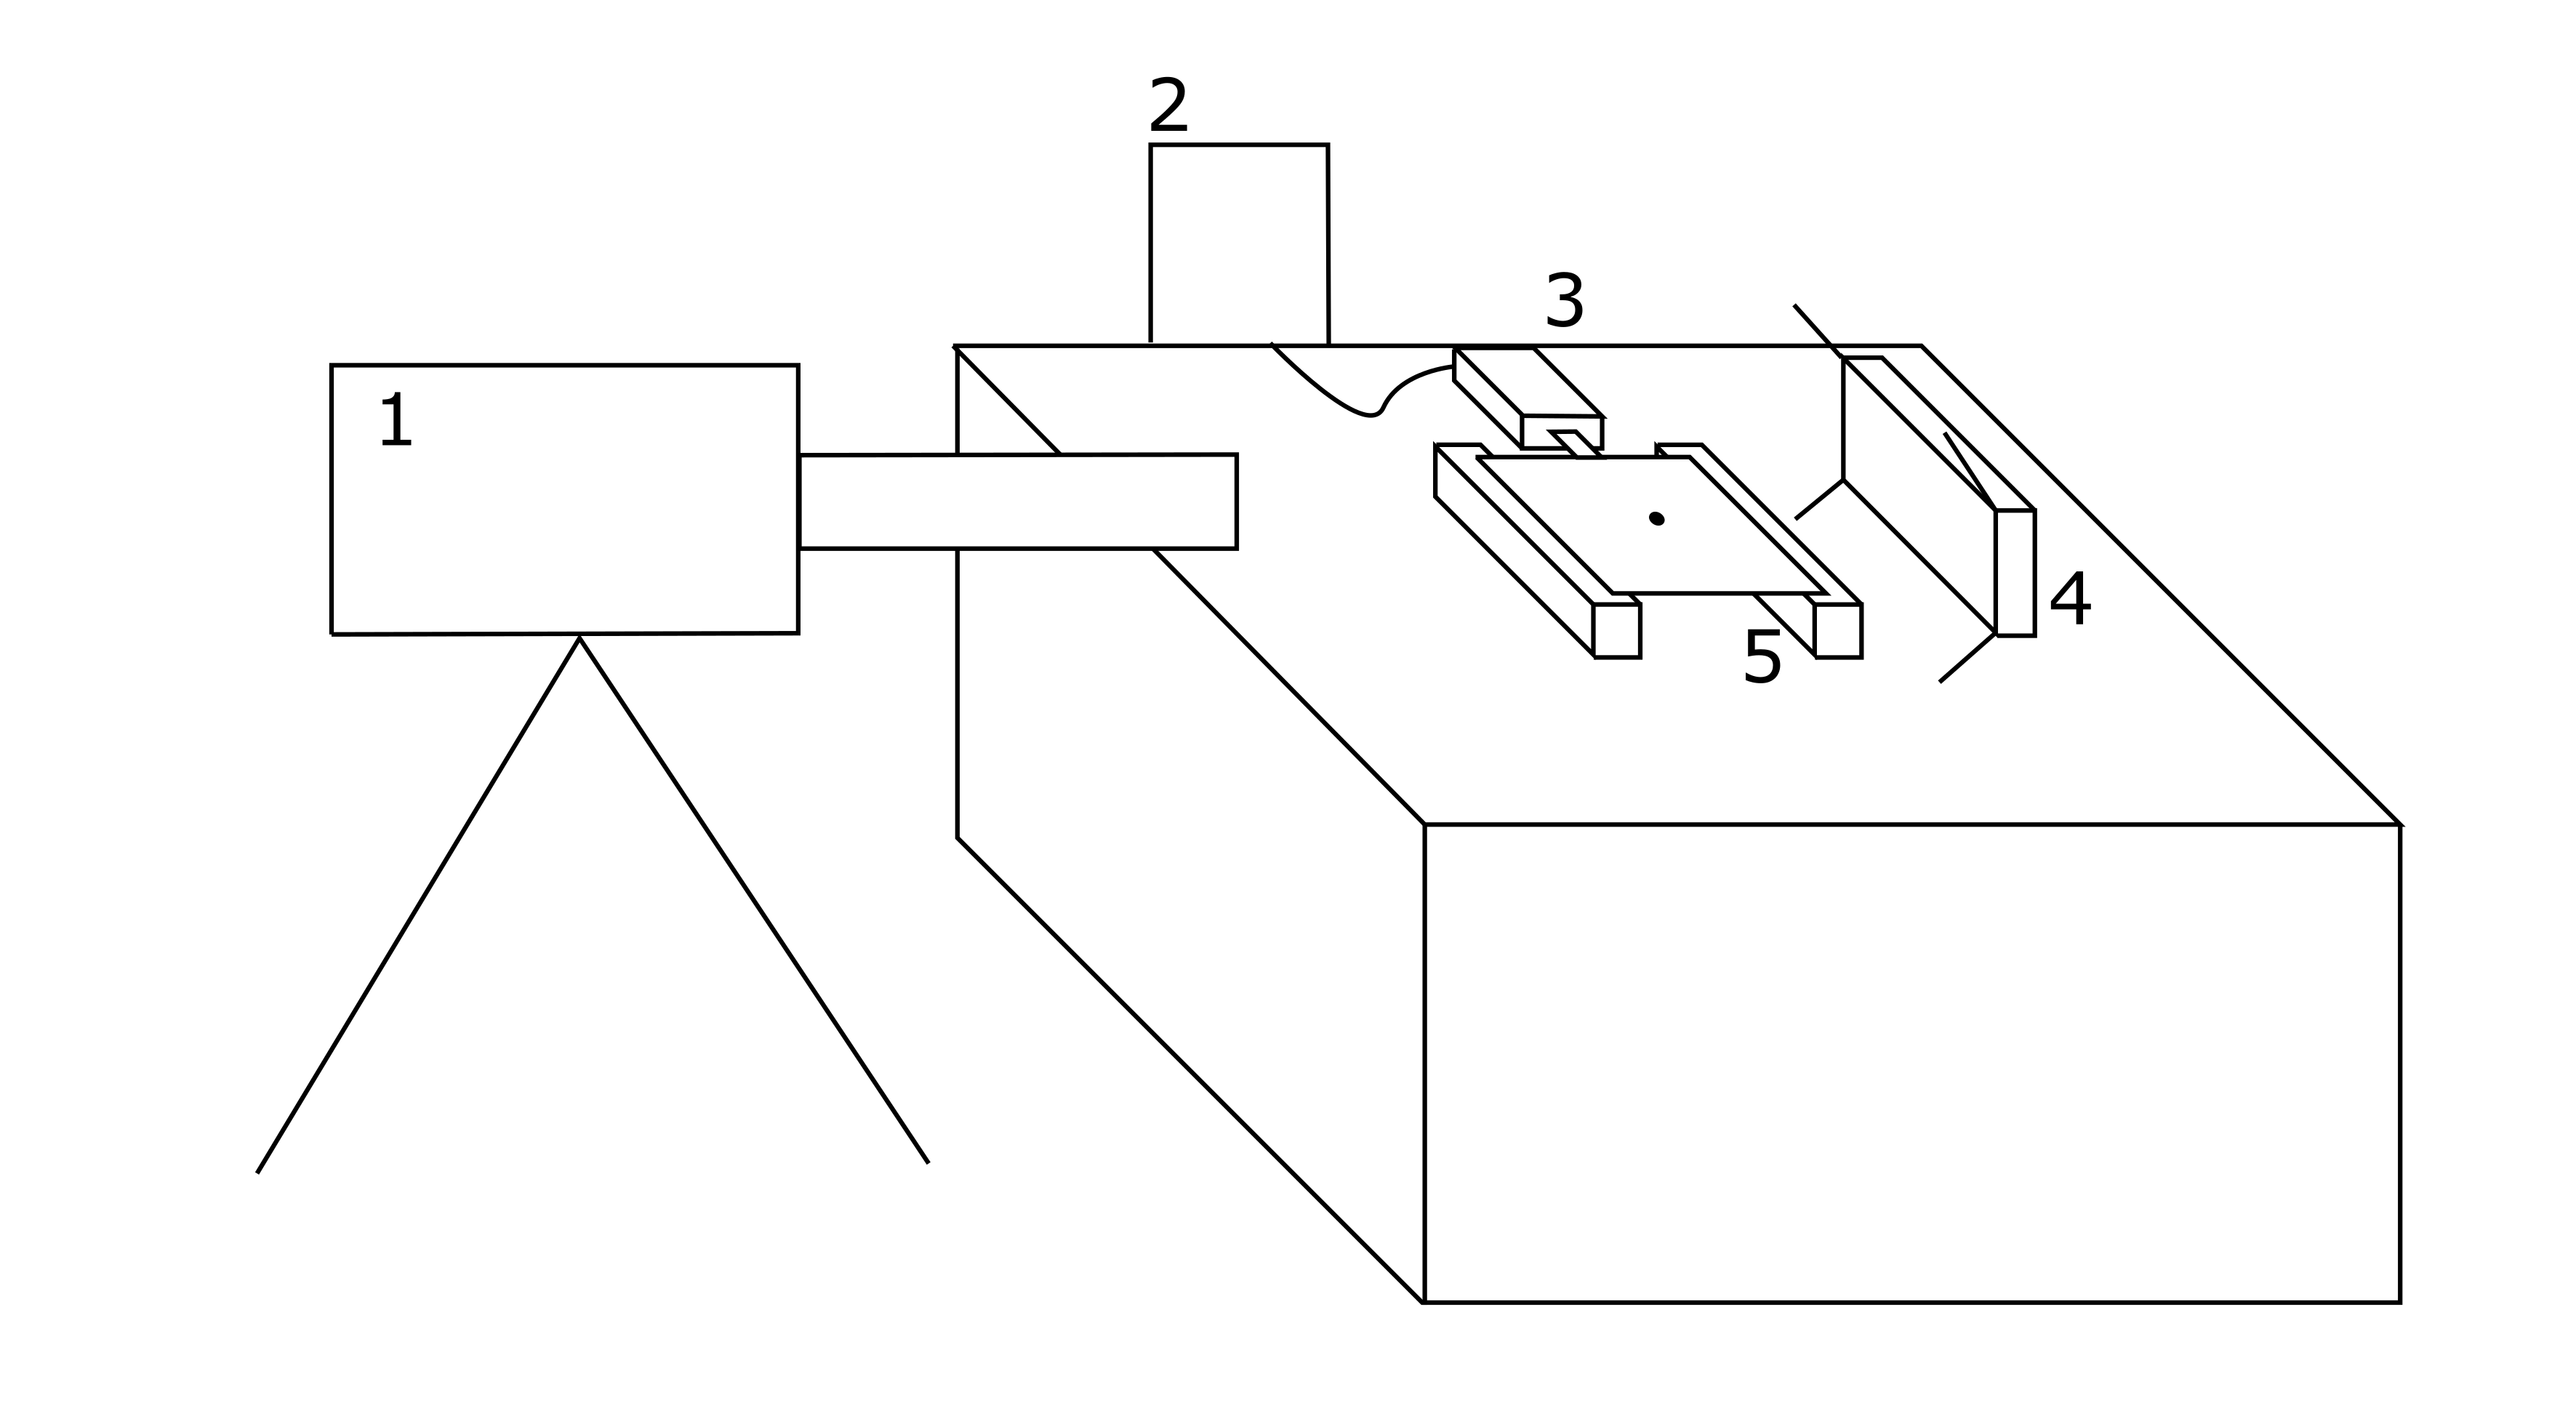
\includegraphics[width=\linewidth]{img/stan.png}
    \caption{Schemat stanowiska}
\end{figure}

Kropla umieszczana była na płytce za pomocą dozownika, który zapewniał jednakowy rozmiar kropli za każdym razem. W eksperymencie używano wody destylowanej.

\newpage
\subsection{Metoda pomiaru}
\noindent Pomiar dokonywany był w następujący sposób:
\begin{enumerate}
    \item umieszczenie kropli na płytce,
    \item uruchomienie silnika z zadaną częstotliwością i amplitudą,
    \item uchwycenie 1 sekundy ruchu płytki z kroplą kamerą
\end{enumerate}

\subsubsection{Umieszczenie kropli na płytce}
Kroplę na płytce ustawiano spuszczając 2 mniejsze krople z stałej wysokości. Ilość wody w pomiarze zawsze była jednakowa. Masę kropli obliczono na podstawie zdjęcia jednej małej kropli spadającej na płytkę, przedstawionym na rysunku 2.2. Znając skalę kamery, obliczono objętość sfery, a następnie przemnożono ją przez gęstość płynu.

\begin{figure}[!h]
    \label{fig:poślizg}
    \centering 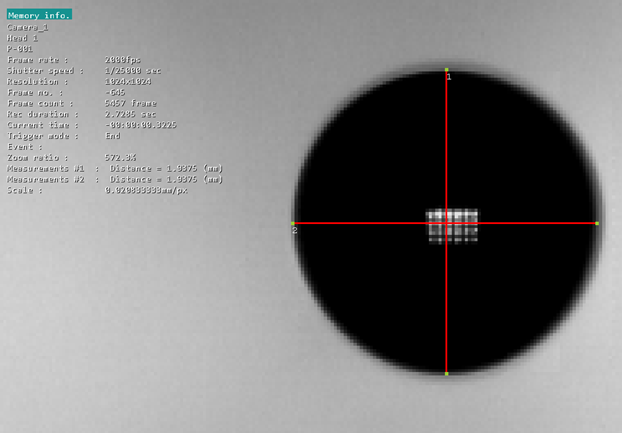
\includegraphics[width=0.8\linewidth]{img/drop.png}
    \caption{Obraz kropli spadającej na płytkę uchwycony kamerą}
\end{figure}

\begin{table}[!h] \centering \label{tab:tabela1}
\begin{tabular} {| c | c | c  |} \hline 
pomiar x & pomiar y	& średnia \\
\hline
2,021 & 1,896 & 1,9585\\
2,021 &	1,854 & 1,9375\\
1,958 &	1,917 &	1,9375\\
1,917 &	1,979 &	1,948\\
1,938 &	1,938 &	1,938\\
\hline
\end{tabular}
\caption{Pomiary średnicy kropli}
\end{table}
Na podstawie 5 pomiarów obliczono średnią średnicę kropli $d = 1,9439 mm$. Masa kropli w eksperymencie wynosiła zatem w każdym pomiarze:
\begin{align*}
    m = 2 \cdot \rho \cfrac{4}{3}\pi\cfrac{d^3}{8} = 7,692 mg
\end{align*}
\subsection{Silnik liniowy}

Płytka z kroplą poruszana jest przez silnik liniowy \textit{Linmot} C1100. Silnik obsługiowany jest przez storownik, który pozwala na wgranie dowolnej krzywej ruchu. W poniższej pracy celem było wygenerowanie drgań o małej amplitudzie, ale wysokiej częstotliwości. W tym celu wygenerowano krzywą opisaną jako $x = A\sin{\omega t}$, pokazanej na rysunku 2.3

\begin{figure}[!h]
    \label{fig:poślizg}
    \centering 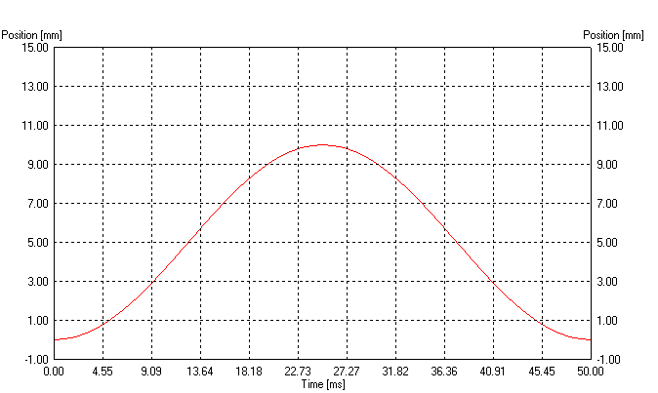
\includegraphics[width=0.8\linewidth]{img/curve.png}
    \caption{Krzywa zadana w silniku liniowym}
\end{figure}

W eksperymencie zdecydowano się testować 3 różne amplitudy.
\begin{itemize}
    \item $1mm$,
    \item $2mm$,
    \item $3mm$.
\end{itemize}

Amplitudy drgań są porównywalne z rozmiarem kropli, ponieważ głównym obszarem zainteresowania była zmienność kątów w zależności od częstotliwości. Częstotliwości dobierane były dla każdej amplitudy osobno, tak aby uzyskać jak najwięcej pomiarów przy granicznej częstotliwości, dla której występował poślizg kropli.\\

Sterownik silnika pozwala na odczyt wielu parametrów ruchu - zadanych i rzeczywistych. Podczas każdego pomiaru zapisywano krzywą rzeczywistego przyspieszenia wózka, w celu odczytania wartości maksymalnej. 

\newpage

\subsection{Ustawienia kamery}





         % Wygodnie jest trzymać każdy rozdział w osobnym pliku.
                            % na nowe wersje, a cały tekst pracy pozostaje nienaruszony.

\newpage % Rozdziały zaczynamy od nowej strony
\section{Summatio}          % Można też pisać rozdziały w jednym pliku.
\lipsum[5-10]

%--------------------------------------------
% Literatura
%--------------------------------------------
\cleardoublepage % Zaczynamy od nieparzystej strony
\printbibliography

%--------------------------------------------
% Spisy (opcjonalne)
%--------------------------------------------
\newpage
\pagestyle{plain}

% Wykaz symboli i skrótów.
% Pamiętaj, żeby posortować symbole alfabetycznie
% we własnym zakresie. Ponieważ mało kto używa takiego wykazu,
% uznałem, że robienie automatycznie sortowanej listy
% na poziomie LaTeXa to za duży overkill.
% Makro \acronymlist generuje właściwy tytuł sekcji,
% w zależności od języka.
% Makro \acronym dodaje skrót/symbol do listy,
% zapewniając podstawowe formatowanie.
% //AB
\vspace{0.8cm}
\acronymlist
\acronym{EiTI}{Wydział Elektroniki i Technik Informacyjnych}
\acronym{PW}{Politechnika Warszawska}
\acronym{WEIRD}{ang. \emph{Western, Educated, Industrialized, Rich and Democratic}}

\listoffigurestoc     % Spis rysunków.
\vspace{1cm}          % vertical space
\listoftablestoc      % Spis tabel.
\vspace{1cm}          % vertical space
\listofappendicestoc  % Spis załączników

% Załączniki
\newpage
\appendix{Nazwa załącznika 1}
\lipsum[1-8]

\newpage
\appendix{Nazwa załącznika 2}
\lipsum[1-4]

% Używając powyższych spisów jako szablonu,
% możesz tu dodać swój własny wykaz bądź listę,
% np. spis algorytmów.

\end{document} % Dobranoc.
